\chapter[Random Forest]{Random Forest aplicado}

\begin{objetivos}
	Ao final desta unidade, o estudante deverá compreender os fundamentos do algoritmo Random Forest; ajustar modelos presença-background para \textit{Dinizia excelsa}; controlar parâmetros para reduzir sobreajuste; avaliar desempenho com dados independentes de teste; comparar desempenho OOB e teste; interpretar importância das variáveis; gerar curvas de resposta parcial; produzir mapas de adequabilidade ambiental; e compreender limitações de algoritmos de aprendizado de máquina em SDM.
\end{objetivos}

\section{Introdução}

Random Forest é um algoritmo de aprendizado de máquina baseado em múltiplas árvores de decisão. Cada árvore é ajustada a partir de uma amostra dos dados e de um subconjunto aleatório das variáveis preditoras. A predição final é obtida pela média das árvores, no caso de regressão ou probabilidade, ou pelo voto majoritário, no caso de classificação \parencite{breiman2001random,cutler2007random,guisan2017habitat}.

Em Modelagem de Distribuição de Espécies, Random Forest é frequentemente utilizado por sua capacidade de representar relações não lineares, interações entre variáveis e respostas ambientais complexas. Entretanto, sua flexibilidade exige cuidado. Modelos muito complexos podem apresentar desempenho aparentemente excelente nos dados de calibração, mas baixa capacidade de generalização espacial ou temporal.

\begin{conceito}[title={\faBook\quad Random Forest em SDM}]
	Random Forest combina muitas árvores de decisão para estimar relações complexas entre ocorrência da espécie e variáveis ambientais. Sua força está na flexibilidade; seu risco está no sobreajuste quando a validação não é adequadamente controlada.
\end{conceito}

\section{Sobreajuste em Random Forest}

Um problema comum em SDM com algoritmos flexíveis é obter métricas muito elevadas, como AUC próxima de 1. Isso pode indicar excelente discriminação, mas também pode ser sintoma de sobreajuste, especialmente quando há autocorrelação espacial, muitos pontos de background, variáveis redundantes ou validação não independente.

Nesta unidade, adotamos quatro estratégias para reduzir esse risco:

\begin{itemize}
	\item separação treino/teste estratificada;
	\item uso de variáveis selecionadas após correlação e VIF;
	\item controle de complexidade por \texttt{mtry}, \texttt{min.node.size} e \texttt{sample.fraction};
	\item comparação entre desempenho OOB e desempenho no conjunto teste.
\end{itemize}

\begin{atencao}[title={\faExclamationTriangle\quad AUC muito alto exige cautela}]
	Em SDM, AUC próximo de 1 nem sempre significa modelo ecologicamente excelente. Pode indicar sobreajuste, viés espacial, background muito fácil de distinguir ou validação não independente.
\end{atencao}

\section{Preparação dos dados}

A base utilizada nesta unidade é a mesma preparada na Unidade 5, com presenças reais de \textit{Dinizia excelsa}, background amostrado dentro da área acessível \(M\) e variáveis ambientais selecionadas na Unidade 4.

\rscriptfile{scripts/unidade08/01_estrutura_pastas.R}

\rscriptfile{scripts/unidade08/02_preparar_dados_rf.R}

\section{Ajuste controlado do Random Forest}

O modelo é ajustado com o pacote \texttt{ranger}, usando probabilidade de presença como saída. Para reduzir sobreajuste, utilizamos valores moderados de \texttt{mtry}, \texttt{min.node.size} maior que o padrão e \texttt{sample.fraction} menor que 1.

\rscriptfile{scripts/unidade08/03_ajustar_rf_dinizia.R}

\begin{figure}[H]
	\centering
	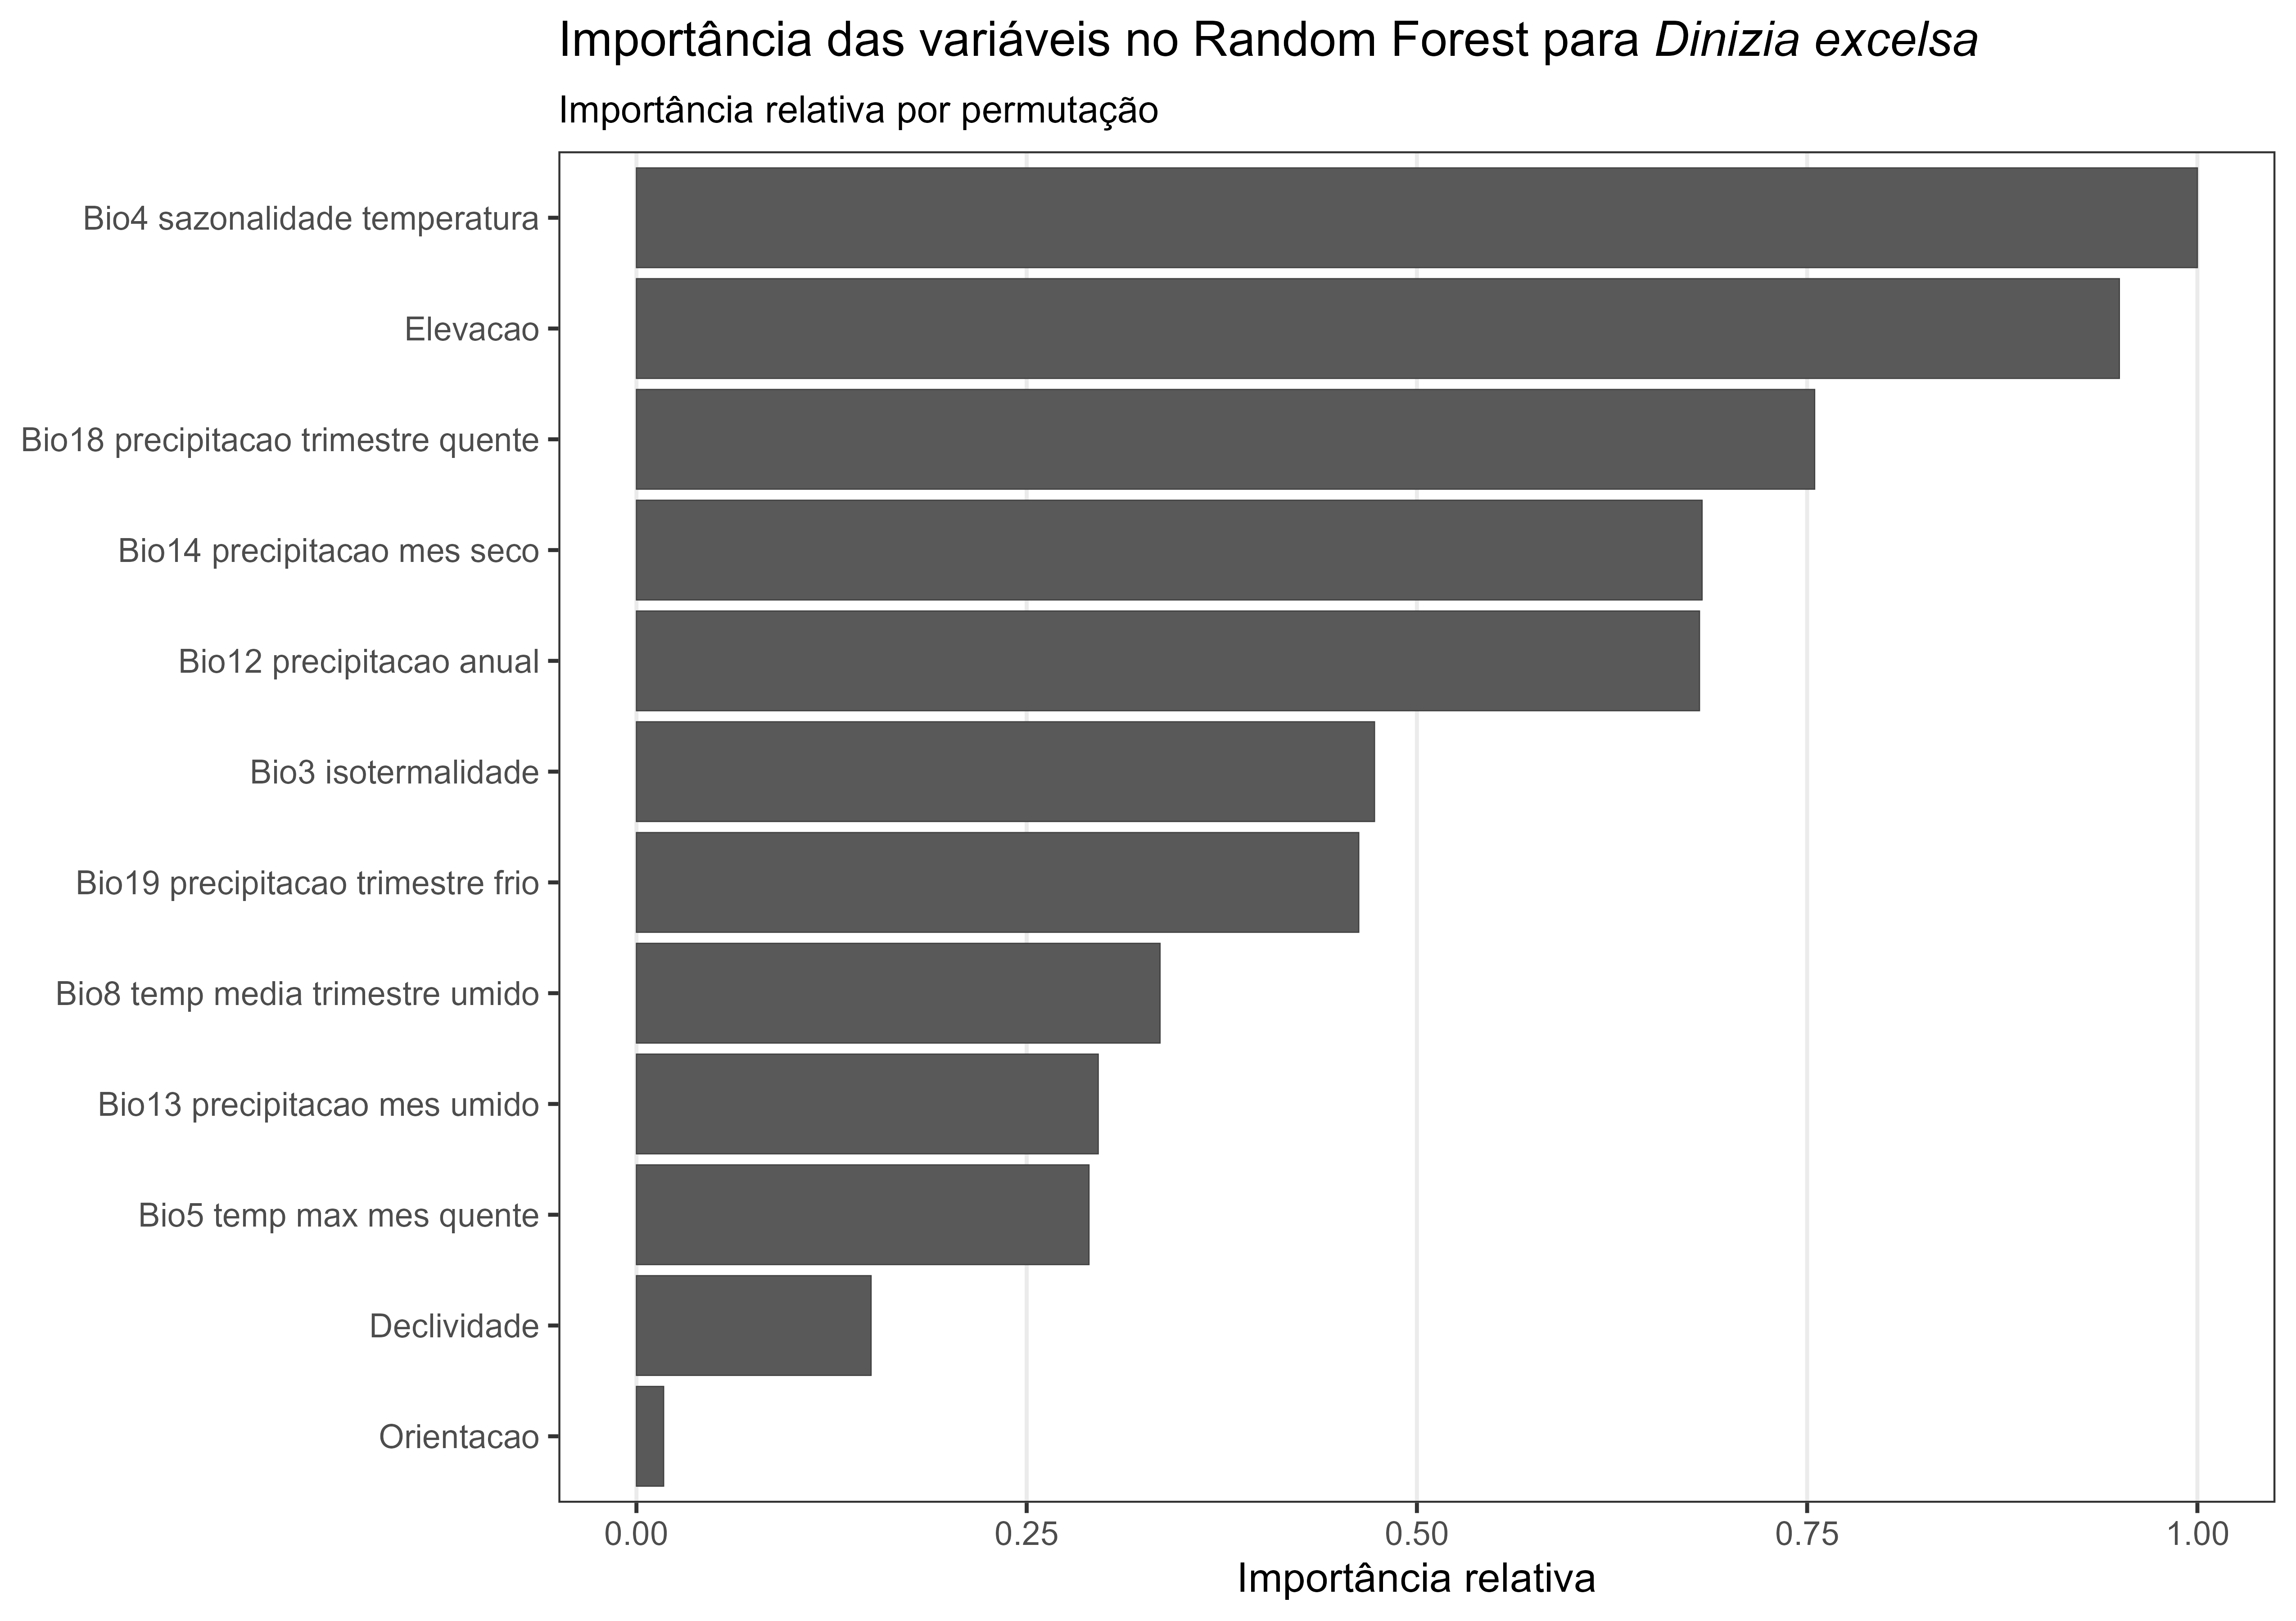
\includegraphics[width=0.86\textwidth]{figuras/unidade08/unidade08_importancia_variaveis_rf.png}
	\caption{Importância das variáveis ambientais no modelo Random Forest ajustado para \textit{Dinizia excelsa}.}
	\label{fig:unidade08_importancia_rf}
\end{figure}

\section{Avaliação do modelo}

O desempenho do Random Forest é avaliado no conjunto teste, não nos dados de treino. Também comparamos AUC OOB e AUC teste. Diferenças muito grandes entre esses valores podem indicar instabilidade ou sobreajuste.

\rscriptfile{scripts/unidade08/04_avaliar_rf_dinizia.R}

\begin{figure}[H]
	\centering
	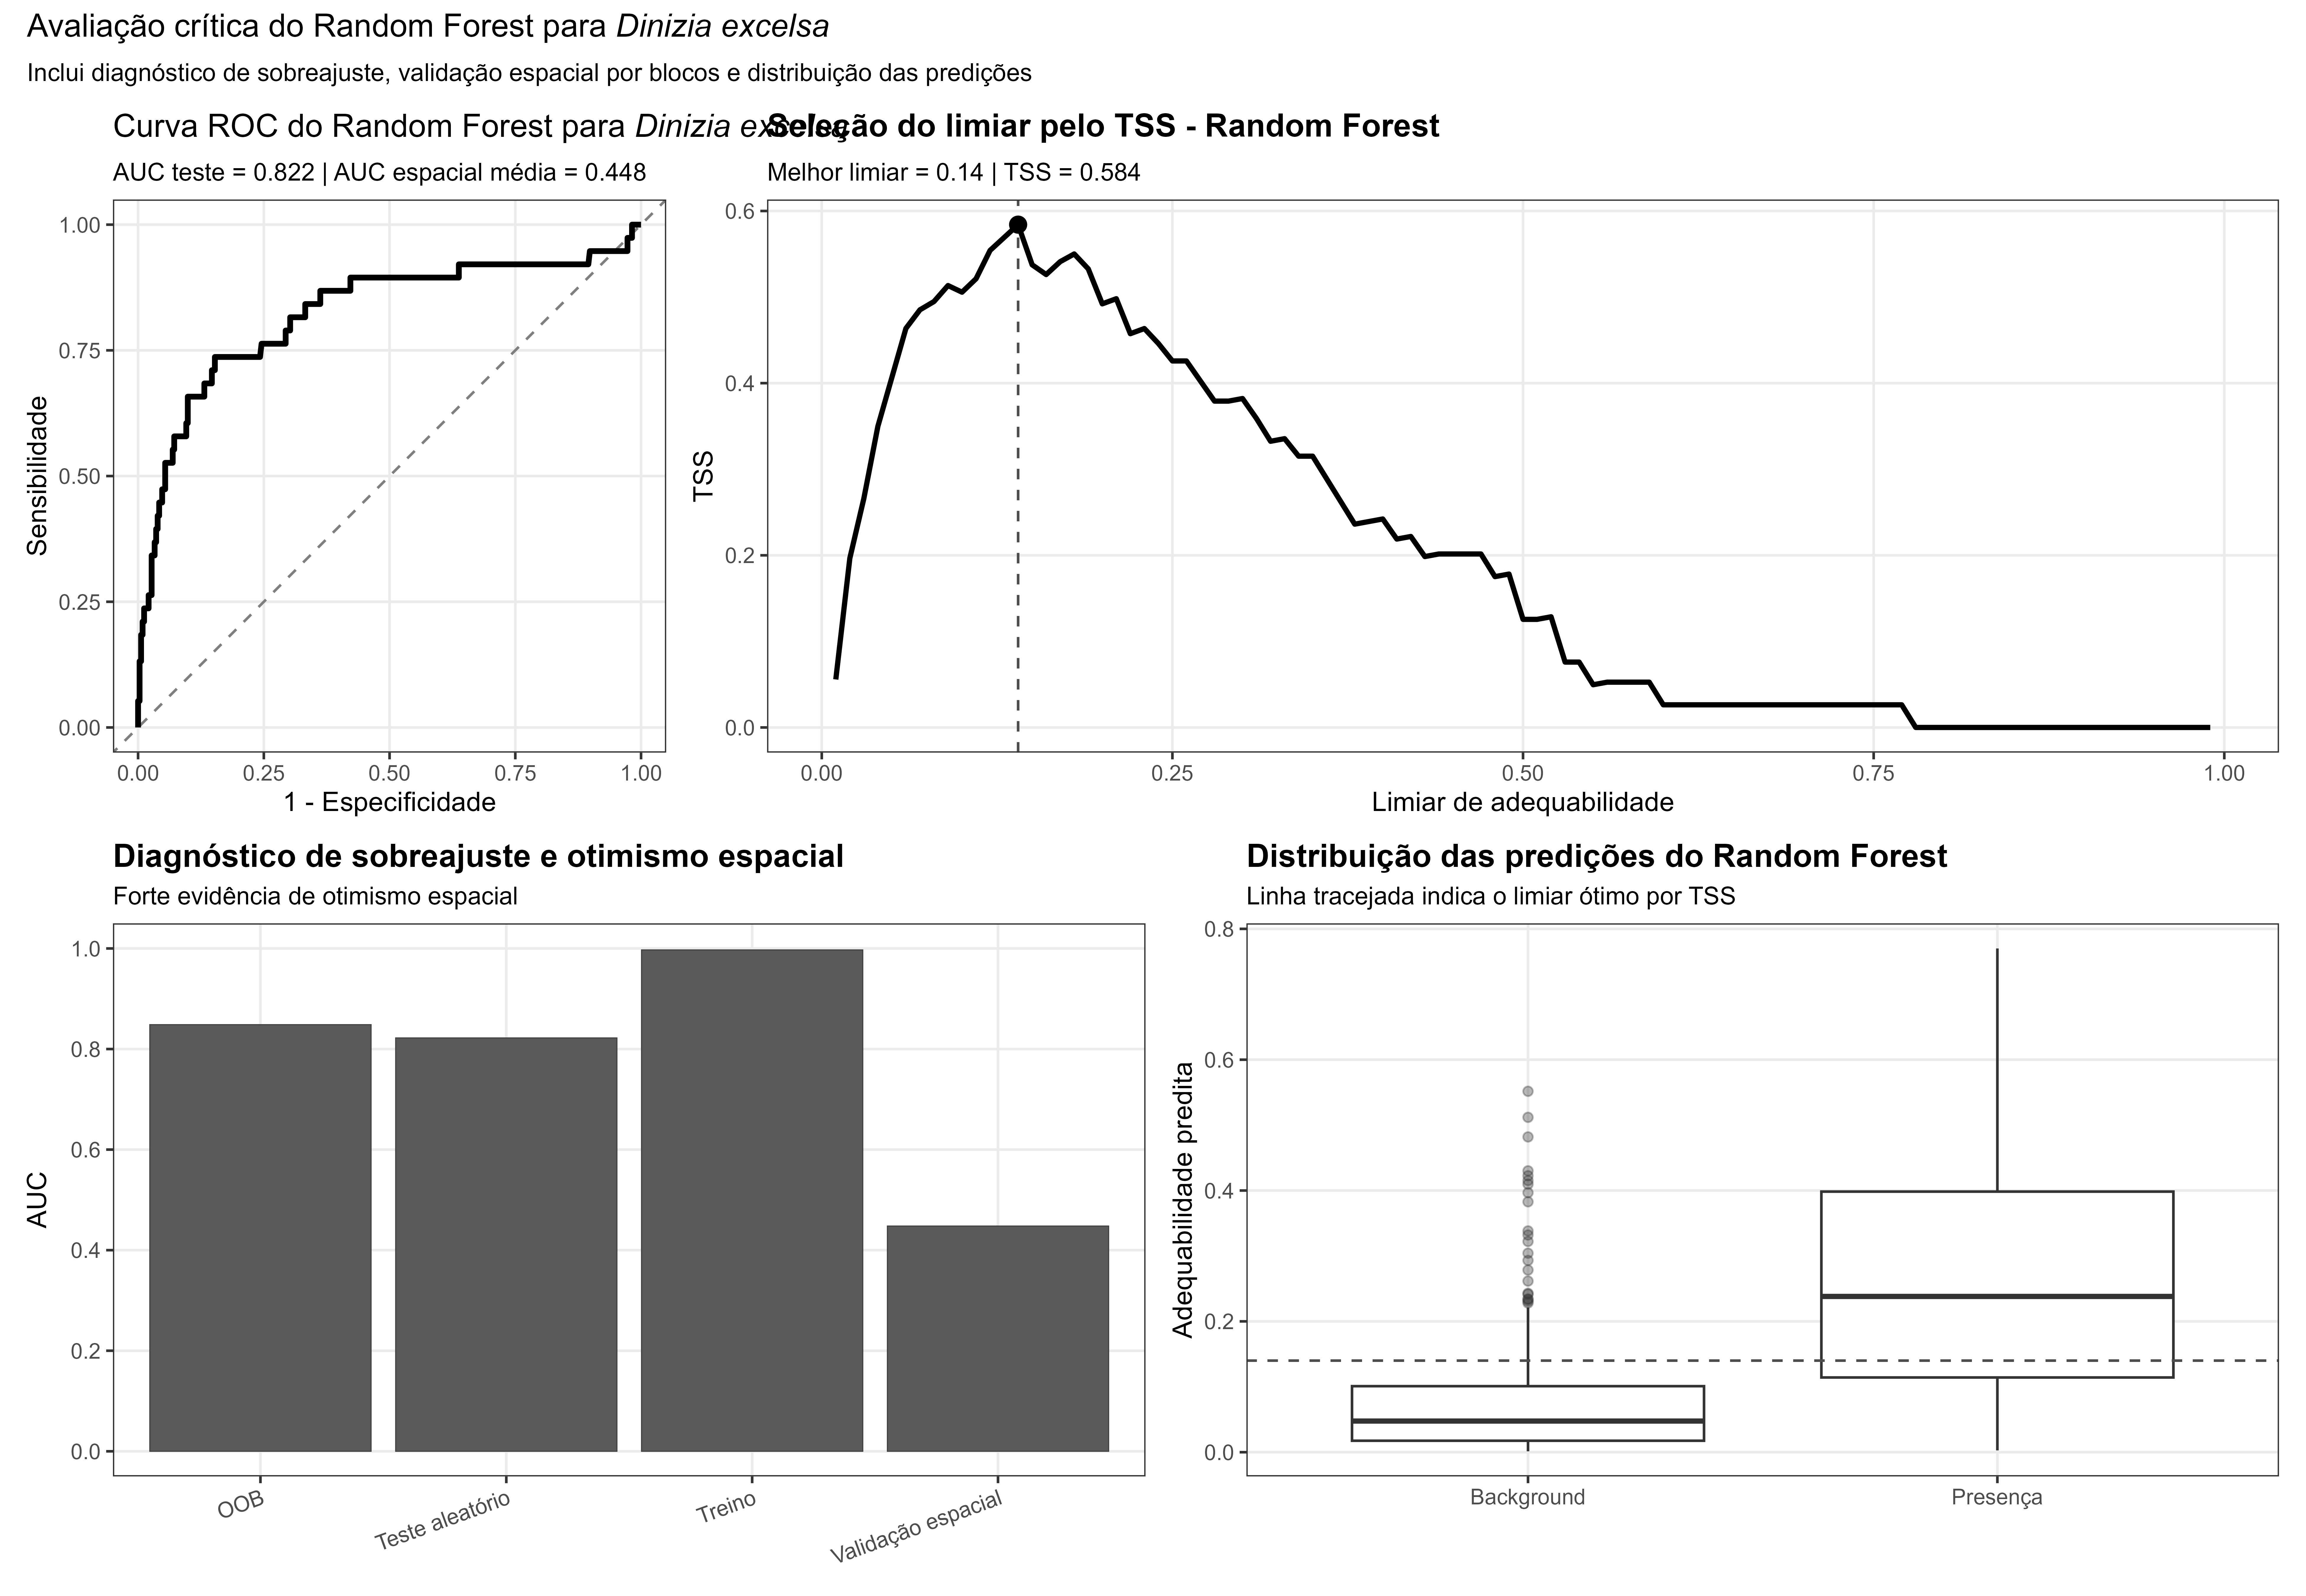
\includegraphics[width=0.78\textwidth]{figuras/unidade08/unidade08_avaliacao_rf_patchwork.png}
	\caption{Curva ROC do Random Forest avaliado no conjunto teste.}
	\label{fig:unidade08_roc_rf}
\end{figure}

\section{Mapa de adequabilidade atual}

Após a avaliação, o modelo é projetado para a área acessível \(M\), produzindo um mapa contínuo de adequabilidade ambiental atual.

\rscriptfile{scripts/unidade08/05_predicao_espacial_rf.R}

\begin{figure}[H]
	\centering
	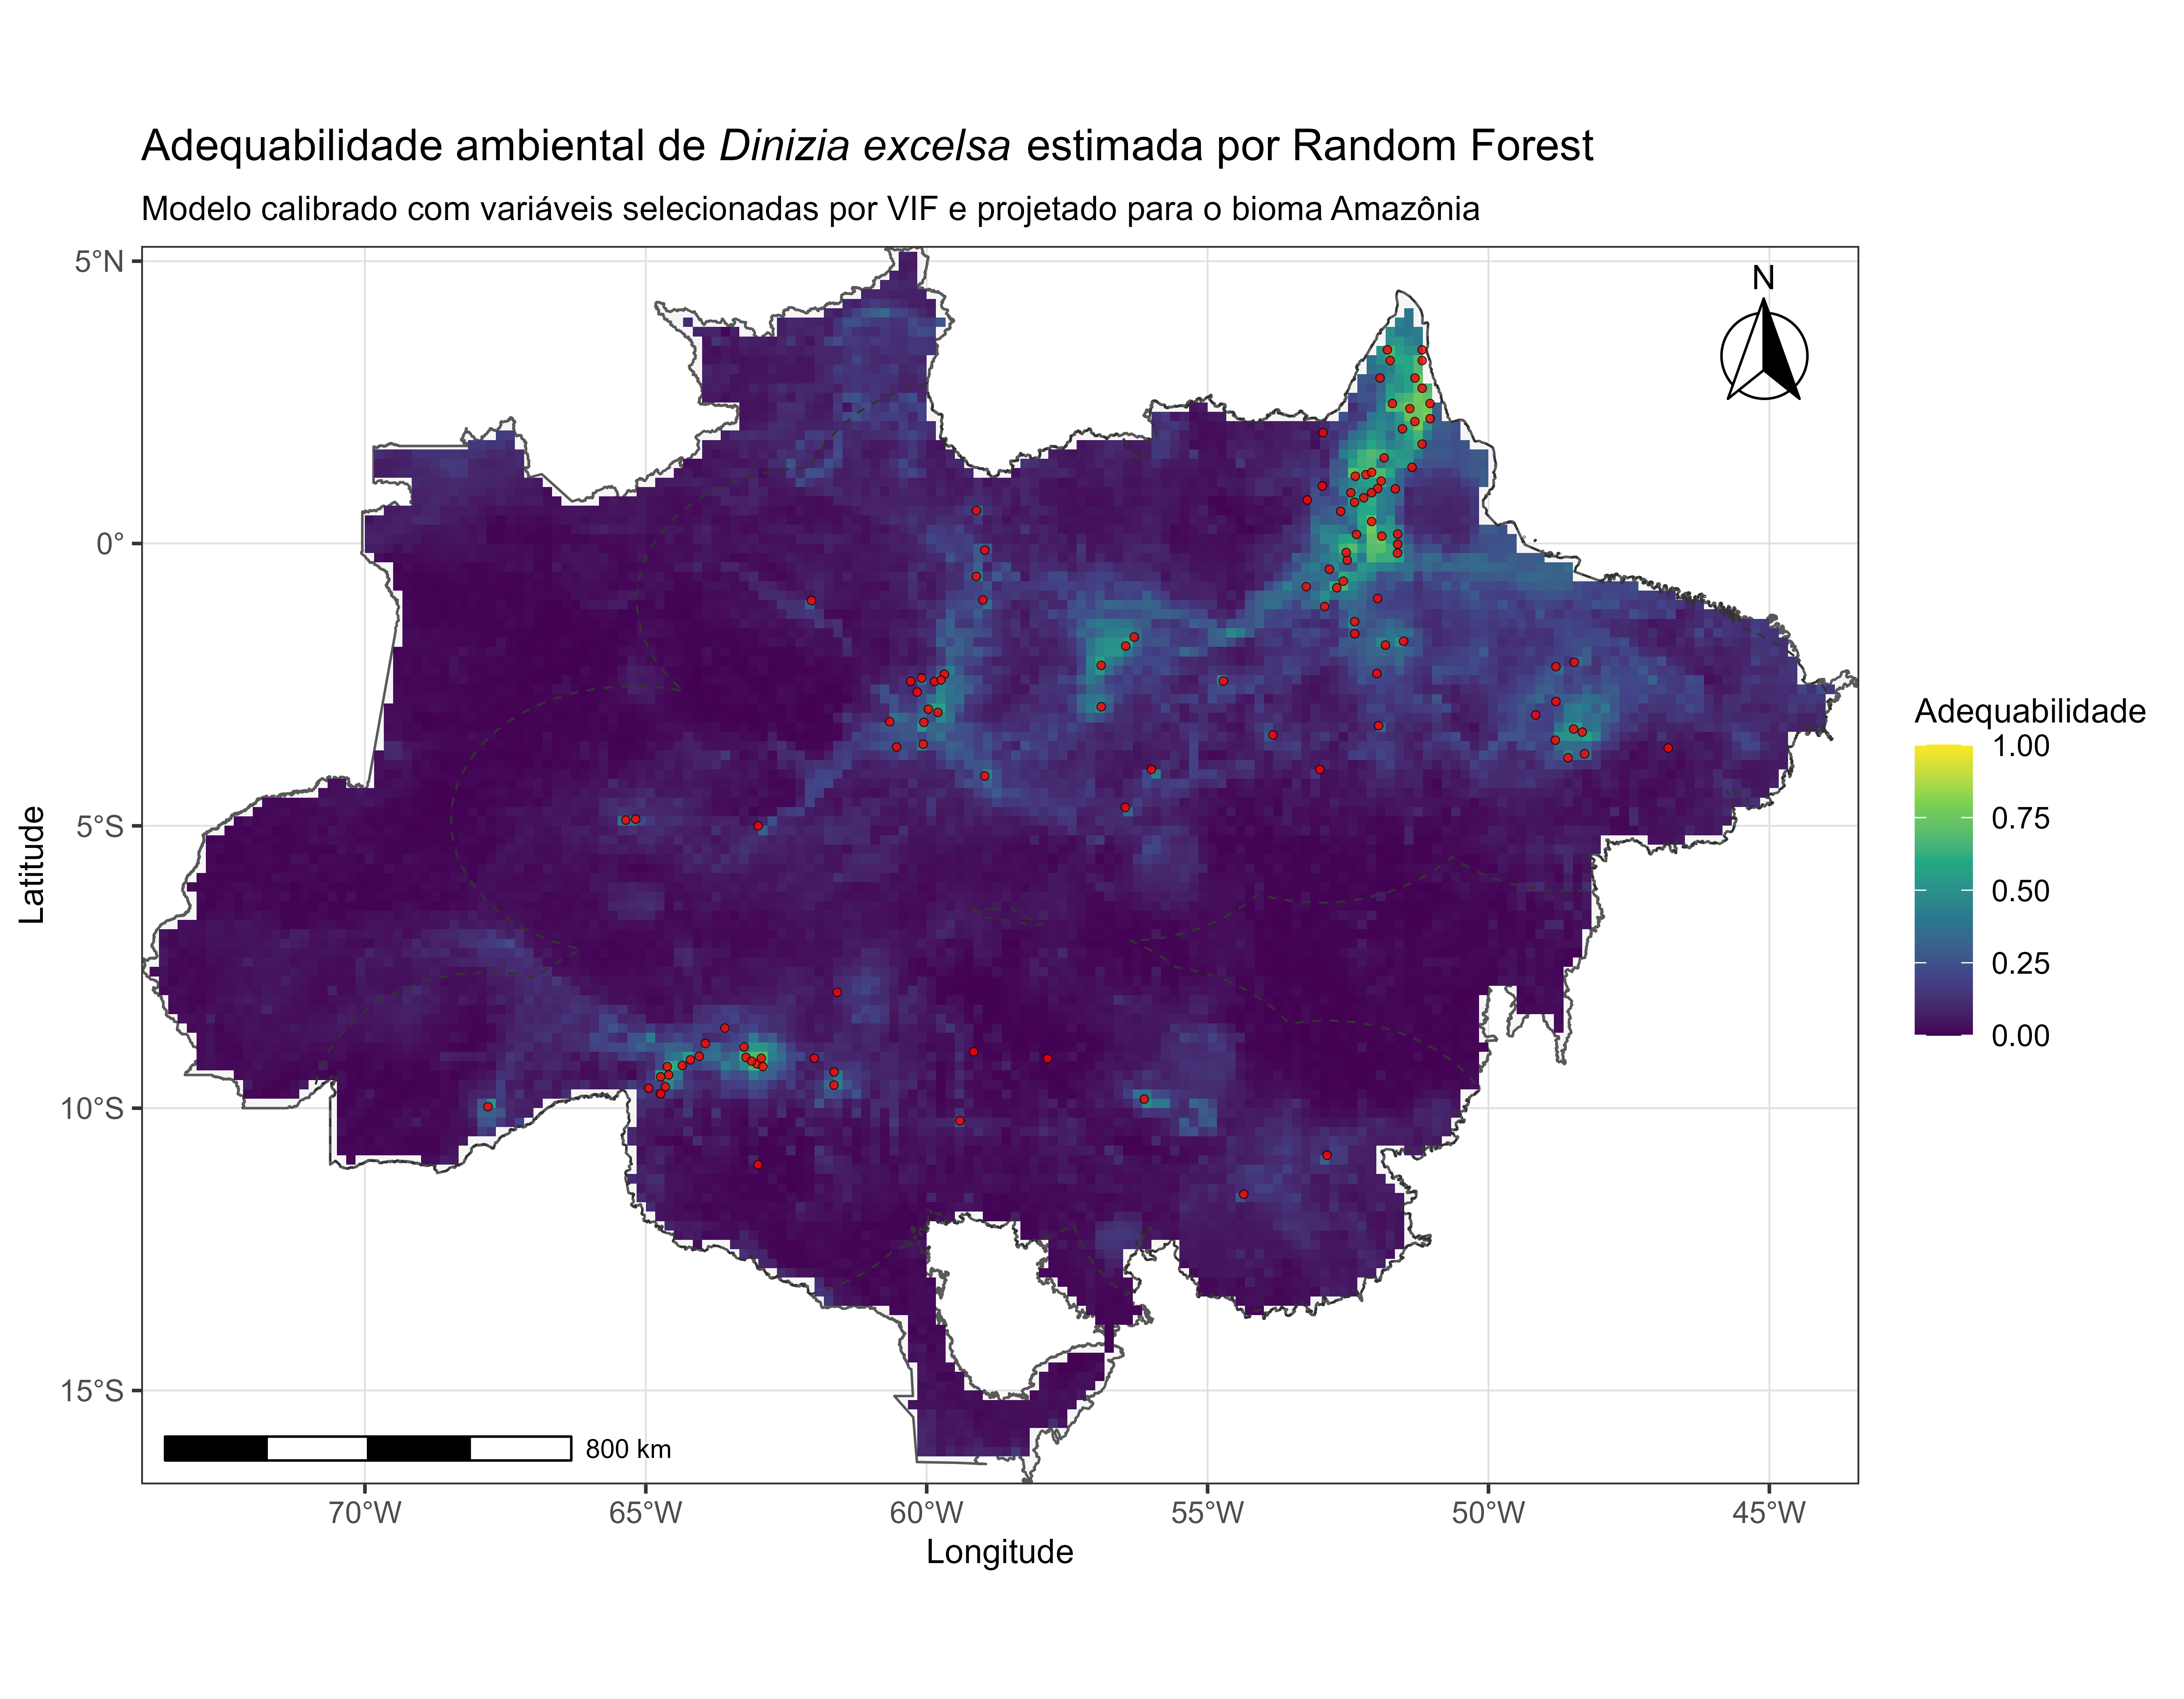
\includegraphics[width=0.88\textwidth]{figuras/unidade08/unidade08_adequabilidade_rf.png}
	\caption{Mapa de adequabilidade ambiental atual de \textit{Dinizia excelsa} estimado por Random Forest dentro da área acessível \(M\).}
	\label{fig:unidade08_adequabilidade_rf}
\end{figure}

\begin{figure}[H]
	\centering
	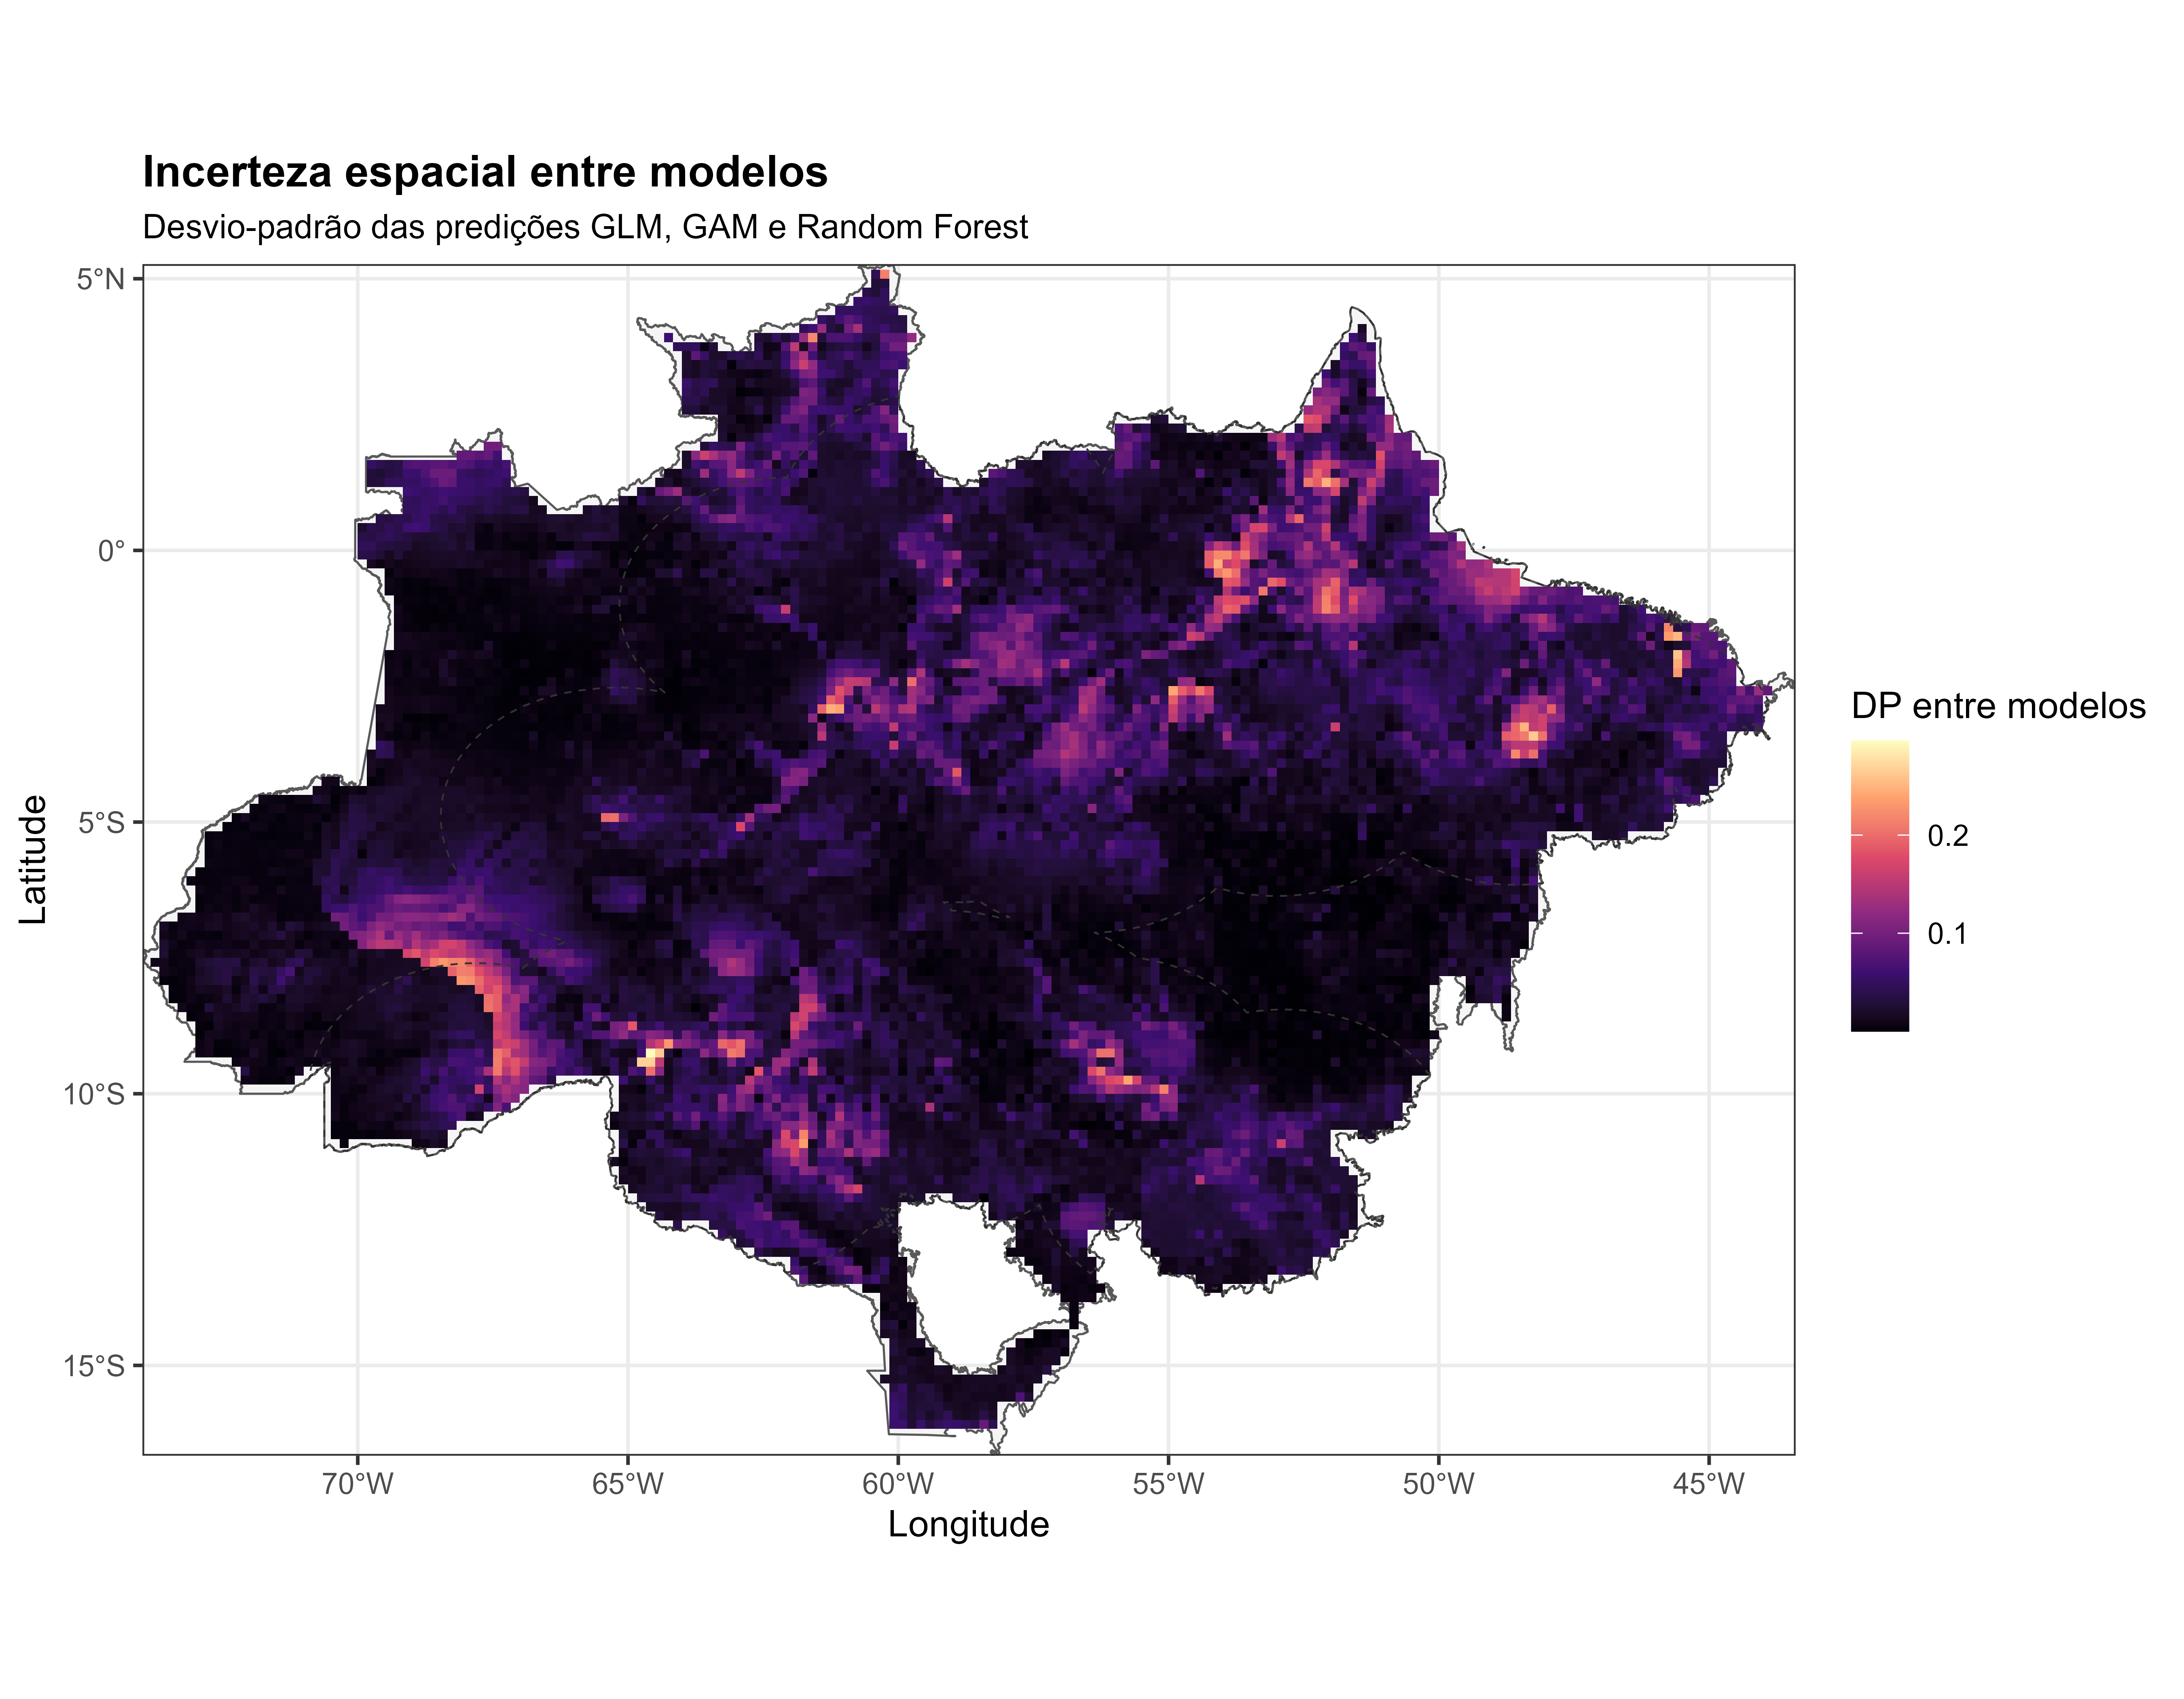
\includegraphics[width=0.78\textwidth]{figuras/unidade08/unidade08_incerteza_sd_glm_gam_rf.png}
	\caption{Mapa de incerteza espacial obtido a partir do desvio-padrão das predições dos modelos GLM, GAM e Random Forest para \textit{Dinizia excelsa}. Valores elevados indicam regiões onde os modelos apresentam maior divergência nas estimativas de adequabilidade ambiental, enquanto valores reduzidos indicam maior consenso entre os algoritmos.}
	\label{fig:unidade08_incerteza_modelos}
\end{figure}

\section{Curvas de resposta parcial}

As curvas de resposta parcial auxiliam na interpretação ecológica do modelo. Em Random Forest, essas curvas não são coeficientes diretos, mas representam a tendência média da predição ao variar uma variável, mantendo as demais constantes.

\rscriptfile{scripts/unidade08/06_curvas_resposta_rf.R}

\begin{figure}[H]
	\centering
	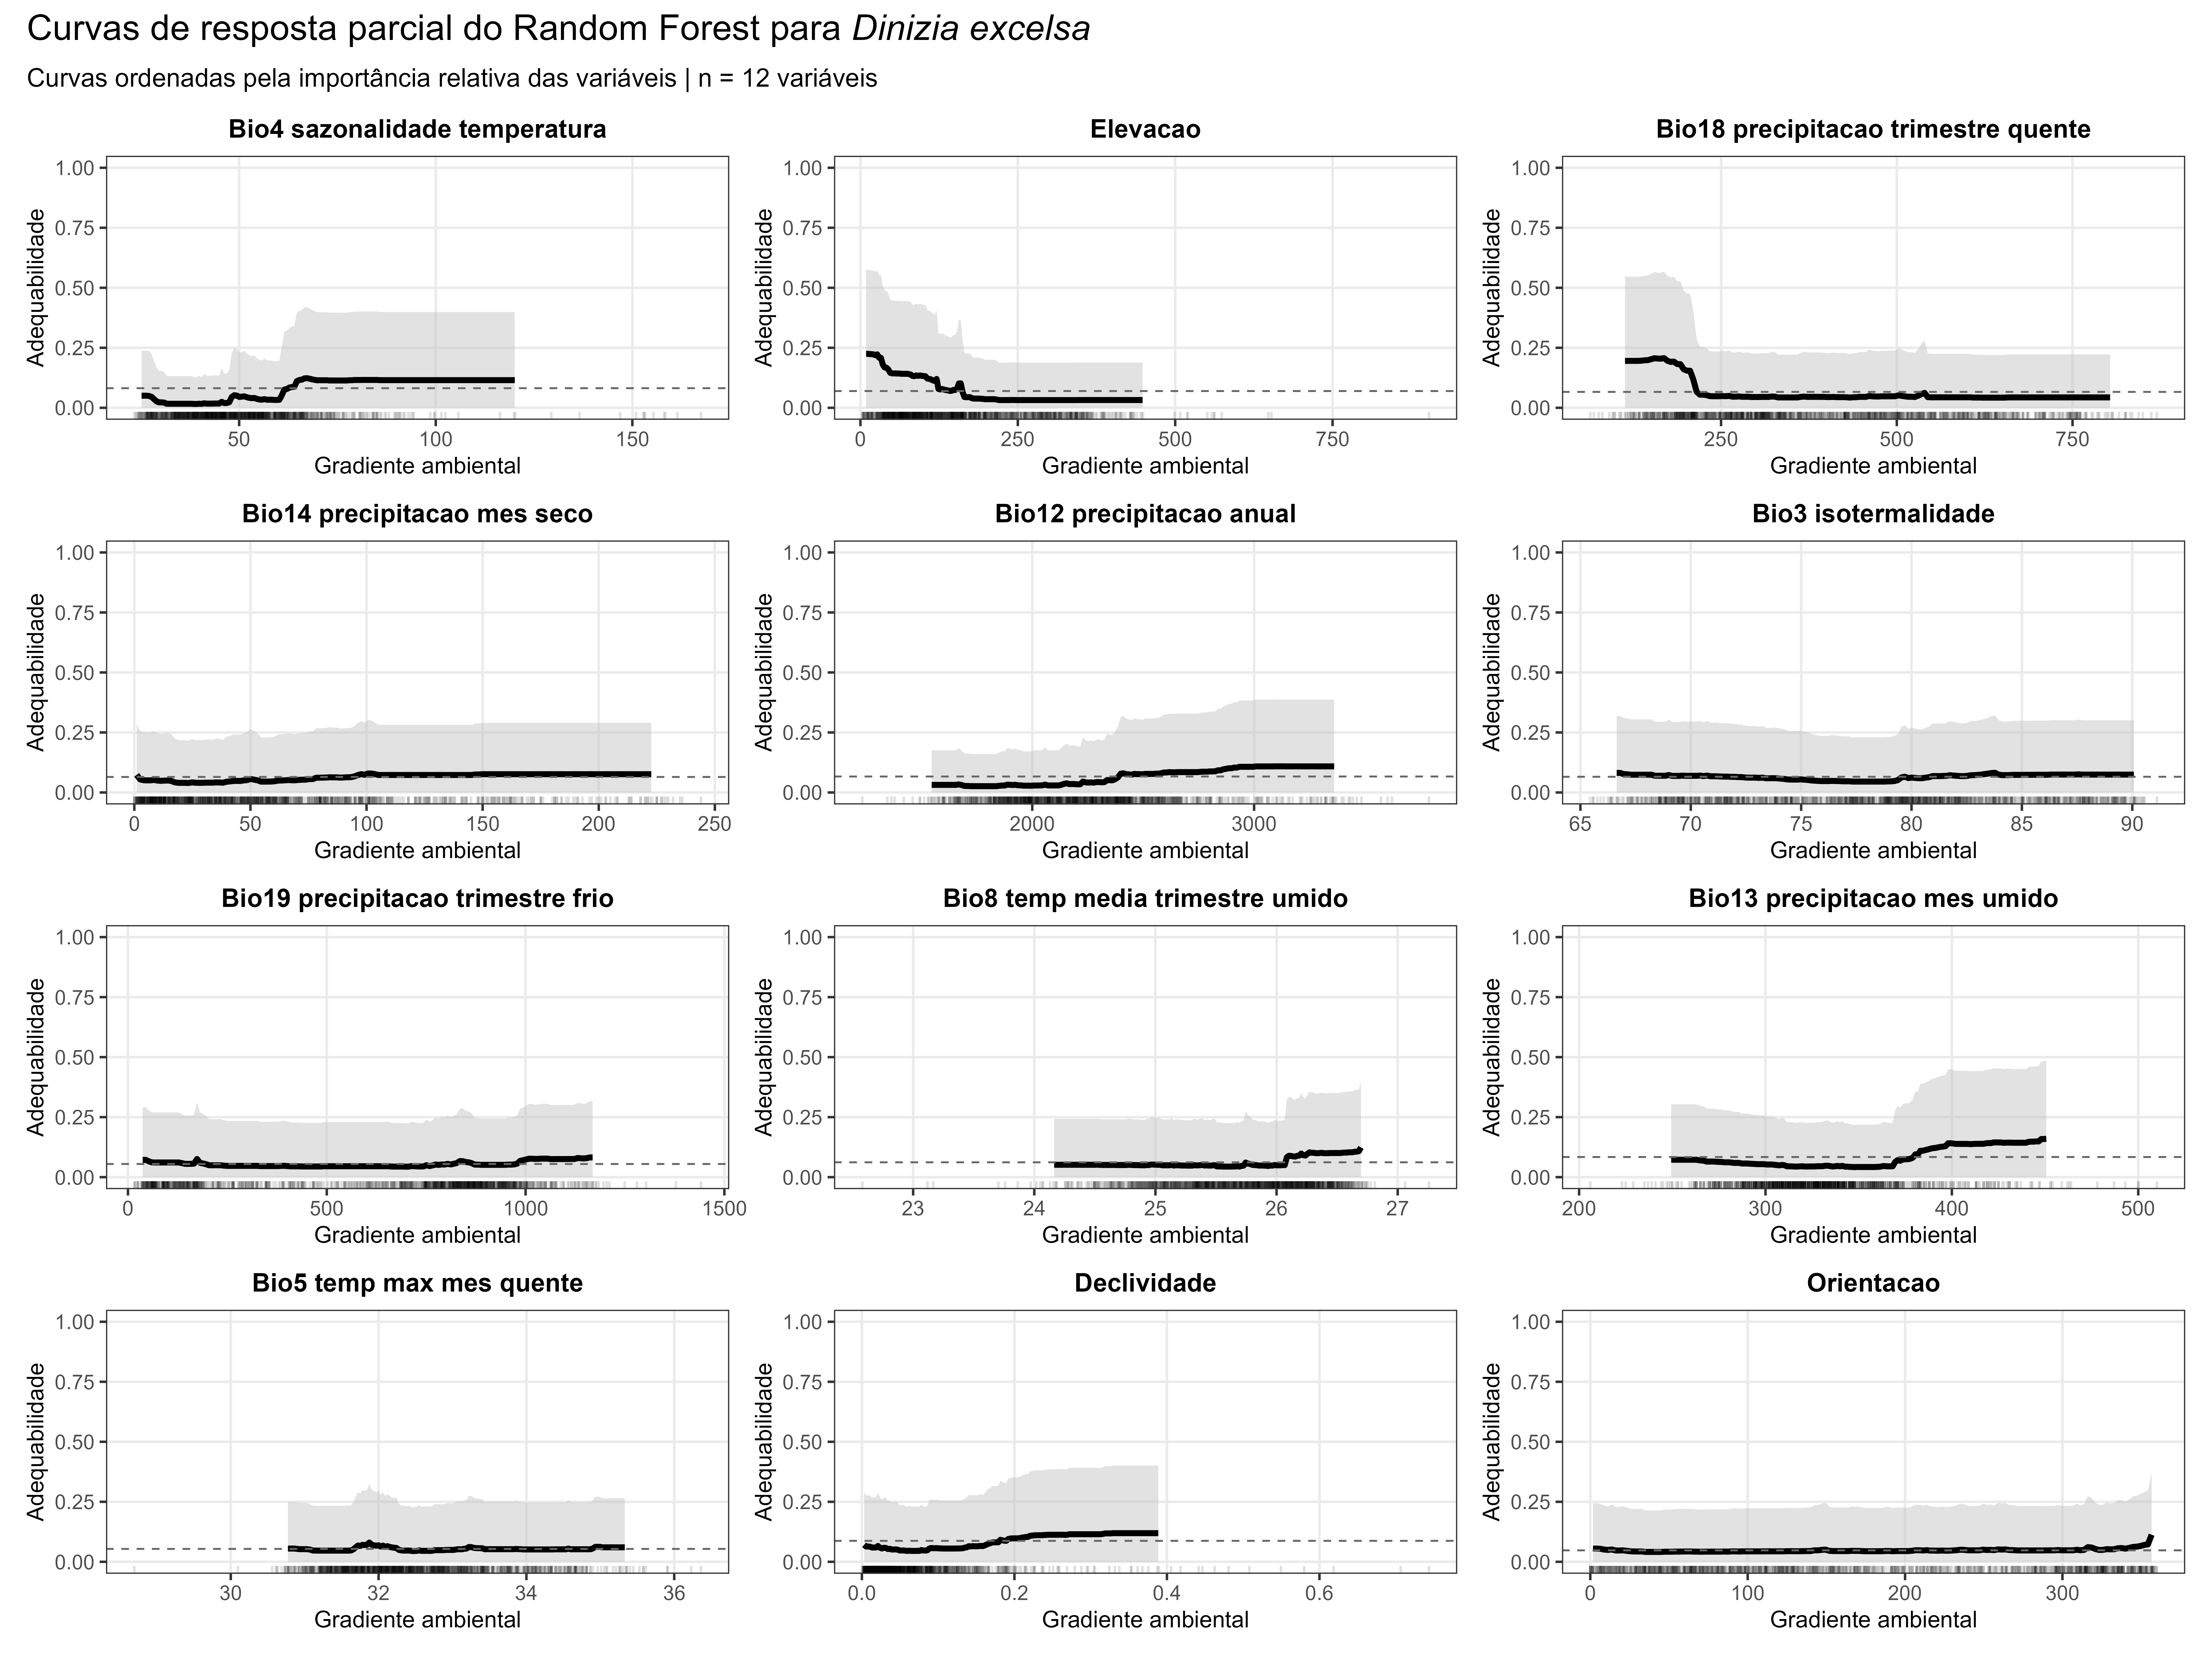
\includegraphics[width=0.96\textwidth]{figuras/unidade08/unidade08_curvas_resposta_rf.png}
	\caption{Curvas de resposta parcial do Random Forest para as variáveis ambientais selecionadas.}
	\label{fig:unidade08_curvas_resposta_rf}
\end{figure}

\section{Comparação com GLM e GAM}

Por fim, comparamos o mapa produzido pelo Random Forest com os mapas gerados por GLM e GAM. Essa comparação mostra como modelos com diferentes níveis de flexibilidade podem produzir padrões espaciais distintos.

\rscriptfile{scripts/unidade08/07_comparar_glm_gam_rf.R}

\begin{figure}[H]
	\centering
	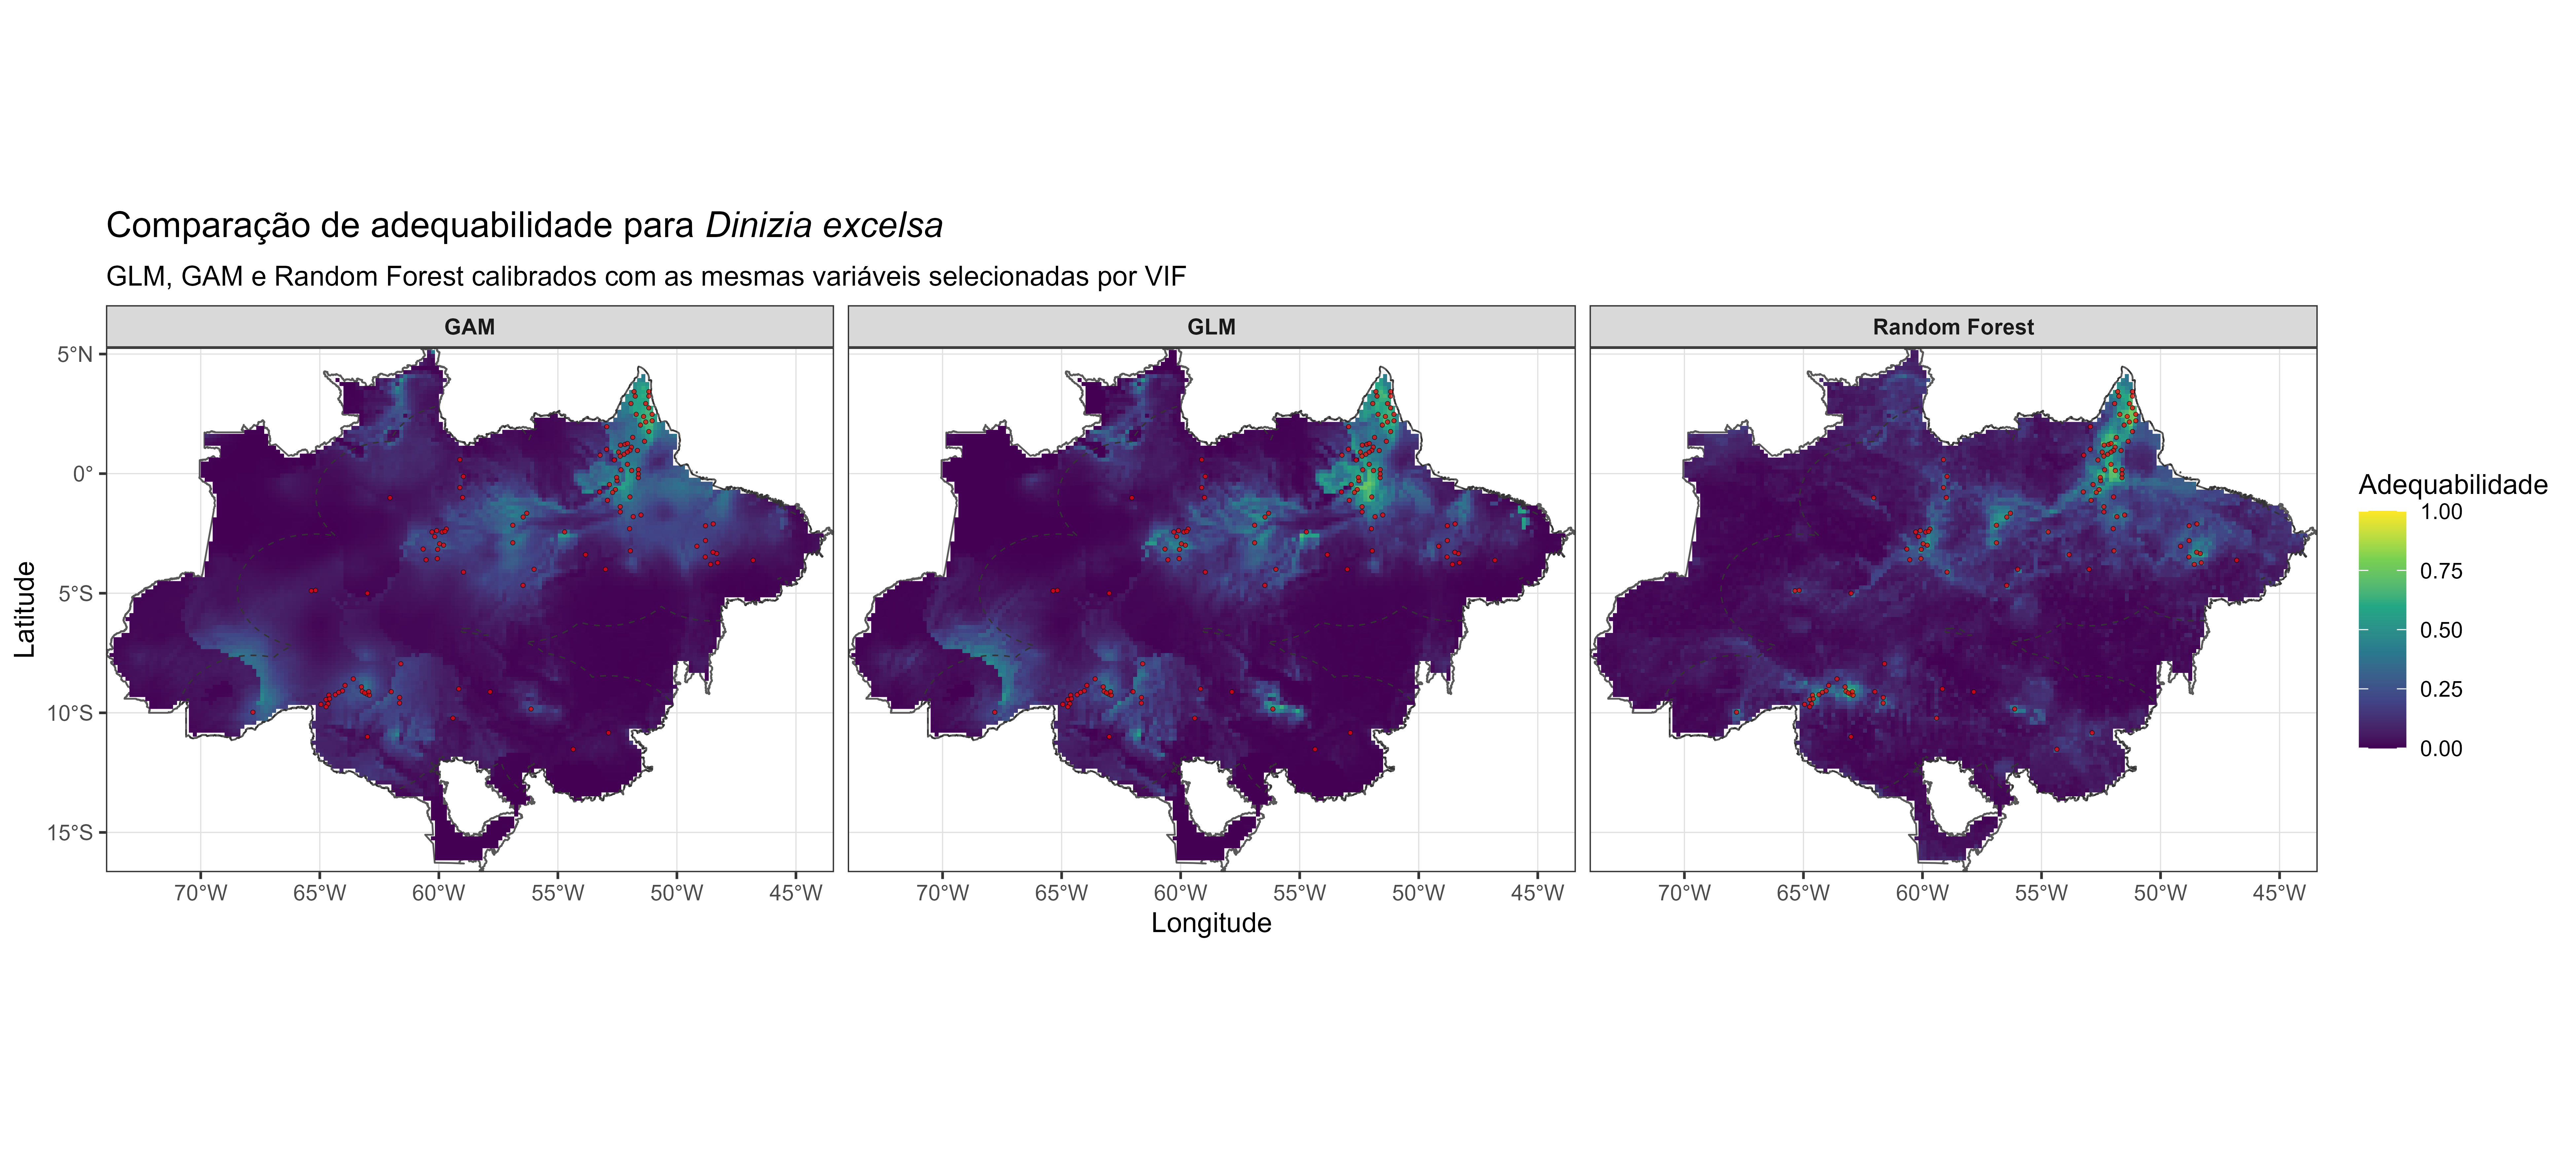
\includegraphics[width=0.96\textwidth]{figuras/unidade08/unidade08_comparacao_glm_gam_rf.png}
	\caption{Comparação entre mapas de adequabilidade estimados por GLM, GAM e Random Forest.}
	\label{fig:unidade08_comparacao_modelos}
\end{figure}

\section{Pipeline completo}

\rscriptfile{scripts/unidade08/08_pipeline_rf.R}

\section{Síntese da unidade}

Random Forest é um algoritmo poderoso para SDM, especialmente quando há relações não lineares e interações entre variáveis. Entretanto, seu uso exige validação cuidadosa. Métricas elevadas devem ser interpretadas em conjunto com diagnóstico de sobreajuste, coerência ecológica, curvas de resposta, distribuição espacial das predições e comparação com modelos mais simples.

\begin{conceito}[title={\faBook\quad Mensagem central}]
	Random Forest pode melhorar o desempenho preditivo, mas não substitui raciocínio ecológico. Um modelo complexo só é útil quando generaliza bem, produz respostas plausíveis e é avaliado de forma independente.
\end{conceito}

\section{Exercícios de fixação}

\begin{enumerate}
	\item Explique como o Random Forest combina múltiplas árvores de decisão.
	\item Por que Random Forest pode capturar relações não lineares?
	\item O que é sobreajuste em SDM?
	\item Por que AUC muito alto pode ser preocupante?
	\item Explique a diferença entre desempenho OOB e desempenho em teste.
	\item Qual o papel de \texttt{mtry}, \texttt{min.node.size} e \texttt{sample.fraction}?
	\item Como curvas de resposta parcial ajudam na interpretação de Random Forest?
\end{enumerate}

% ============================================================
% UNIDADE 9
% ============================================================

